\documentclass[../Main.tex]{subfiles}

\begin{document}

\begin{justify}
En este capítulo se presenta toda la información recolectada y considerada como relevante en relación con la generación de texto y la generación de respuesta a preguntas.
\end{justify}

\section{Introducción}
\begin{justify}
Se ha elaborado una tabla que consiste en cincuenta (50) documentos, principalmente artículos de los cuales se ha recolectado información relevante de cada uno con el fin de identificar las técnicas y algoritmos usados en investigaciones, desarrollo de modelos/sistemas, implementaciones u otros.
\end{justify}

\begin{justify}
La elección de documentos se ha dividido en dos tipos de tareas principales de Procesamiento de Lenguaje Natural (PLN), la primera generación de texto (Text Generation) y la segunda generación de respuestas a preguntas (Question Answering), veinticuatro y veintiséis documentos respectivamente.
\end{justify}

\begin{justify}
Los documentos seleccionados en su mayoría son del año 2008 hasta el presente, esta consideración se tuvo debido al acelerado avance en el campo de NLP hecho por investigadores, con ello el uso de técnicas más sofisticadas y mejores resultados en experimentos realizados.
\end{justify}

\begin{justify}
La información recolectada e identificada como relevante para el trabajo actual, será fundamental para la implementación del modelo adaptado que generará exámenes de Inglés, a continuación se adjunta la tabla elaborada y posteriormente su análisis.
\end{justify}

\subsection{Documentos recolectados}
\begin{justify}
En esta sección se presenta una parte de los cincuenta (50) documentos recolectados, se tuvo en cuenta información relevante como la siguiente:

\begin{itemize}
	\item Técnicas de Procesamiento de Lenguaje Natural\par

	\item Ventajas\par

	\item Desventajas \par

    \item Logros \par
    
    \item Trabajos futuros \par
    
    \item Otros \par
\end{itemize}\par
\end{justify}

\par

\begin{table}[H]
\begin{Center}
	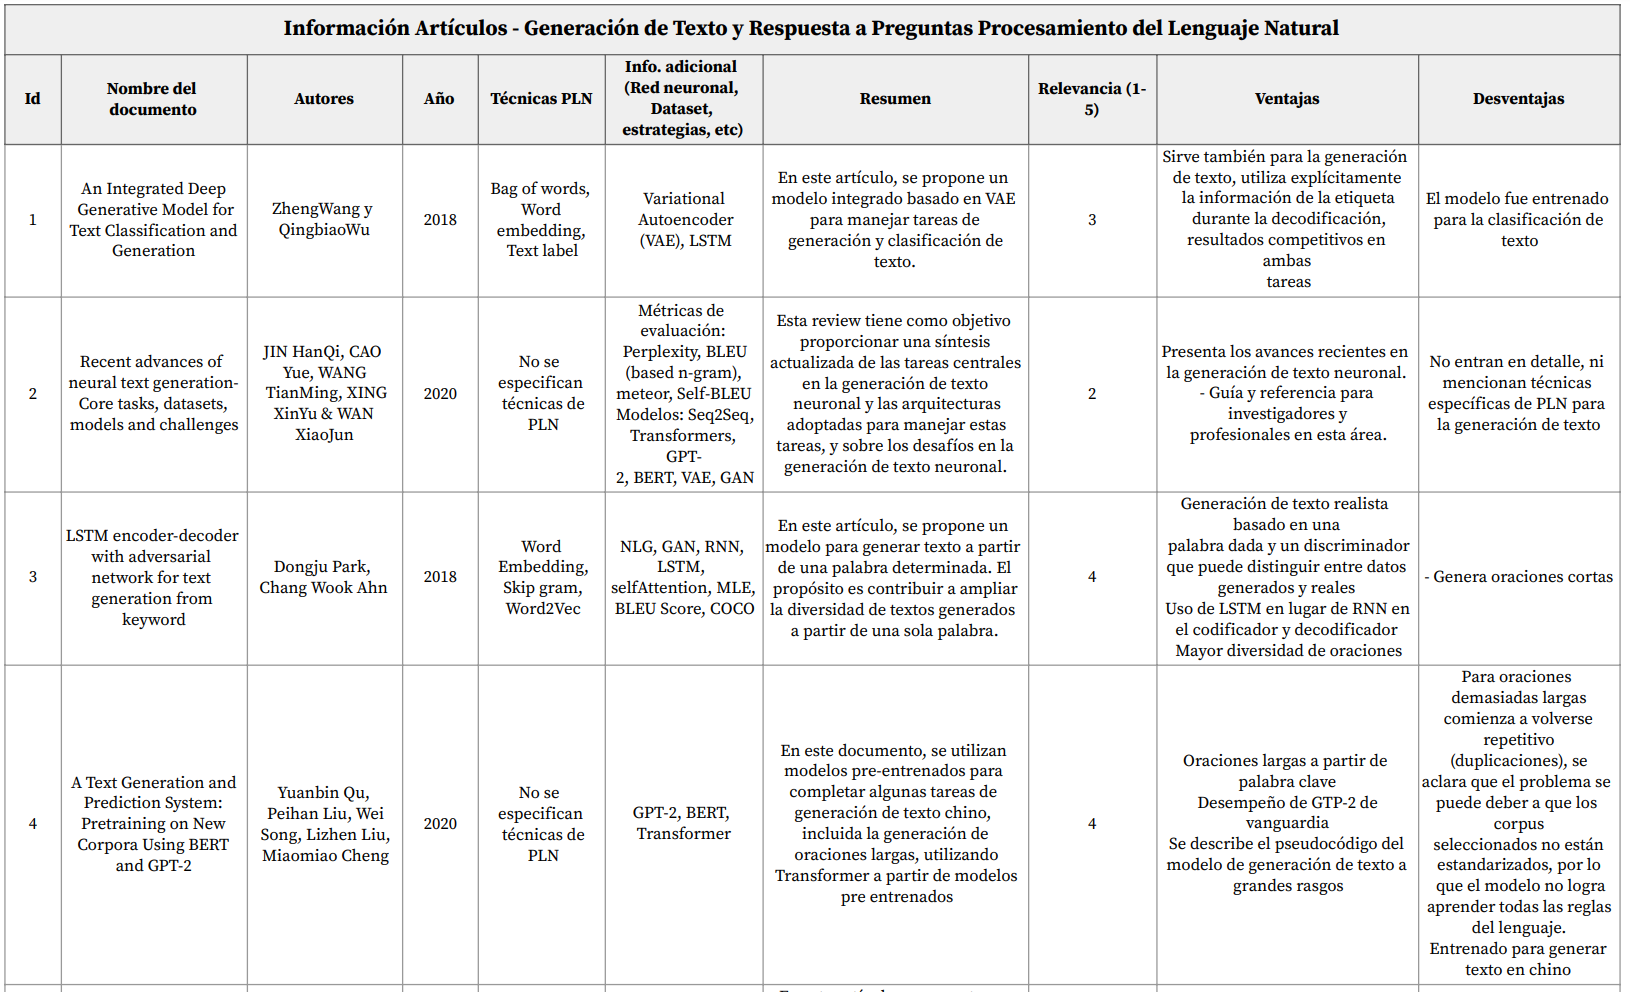
\includegraphics[width=6.4in,height=3.4in]{Images/InicioTablaPapers.png}
\caption{Tabla documentos recolectados}
Fuente: Elaboración propia
\label{tab:table1}
\end{Center}
 \end{table}

La tabla completa se encuentra en los anexos.

\subsection{Algoritmos recolectados}
\begin{justify}
En esta sección se presenta una parte de los diez (10) algoritmos recolectados, se tuvo en cuenta información relevante de manera similar al ítem 3.1.1.
\end{justify}

\begin{table}[H]
\begin{Center}
	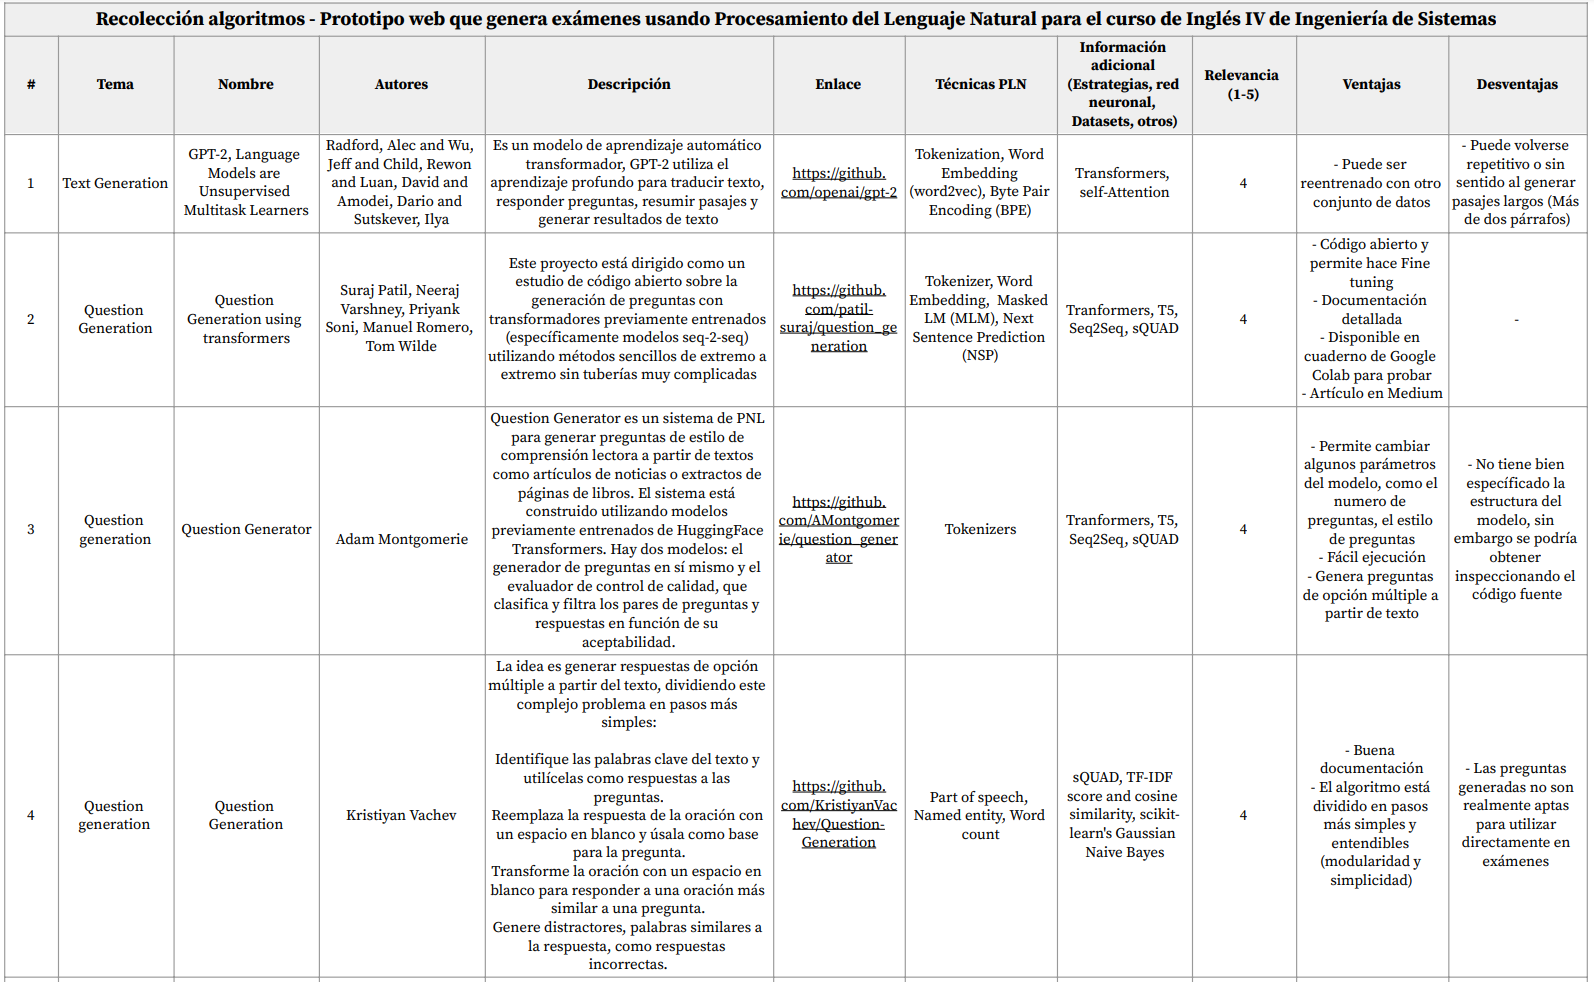
\includegraphics[width=6.4in,height=3.4in]{Images/InicioTablaAlgoritmos.png}
    \caption{Algoritmos recolectados}
    Fuente: Elaboración propia
    \label{fig:section}
\label{tab:table1}
\end{Center}
\end{table}

La tabla completa se encuentra en los anexos.

%\newgeometry{left=0in,right=0in,top=0in,bottom=0.25in}
%\begin{landscape}
%\newpage
%\tiny{
%\subfile{../../Tables/tablaPapers}
%}
%\end{landscape}
%\restoregeometry % restores the margins after frontpage

\subsection{Análisis}

\begin{justify}
De acuerdo a la relevancia de cada documento se le ha asignado un valor de uno (1) a cinco (5) a consideración basándose en ventajas, desventajas, logros, entre otros, siendo cinco (5) muy relevante y uno (1) poco relevante. De acuerdo con el año de publicación se evidencia que después de haber realizado la selección de documentos, los publicados recientemente son los más relevantes en cuanto a resultados obtenidos.\par
\end{justify}

\begin{figure}[H]
	\begin{Center}
		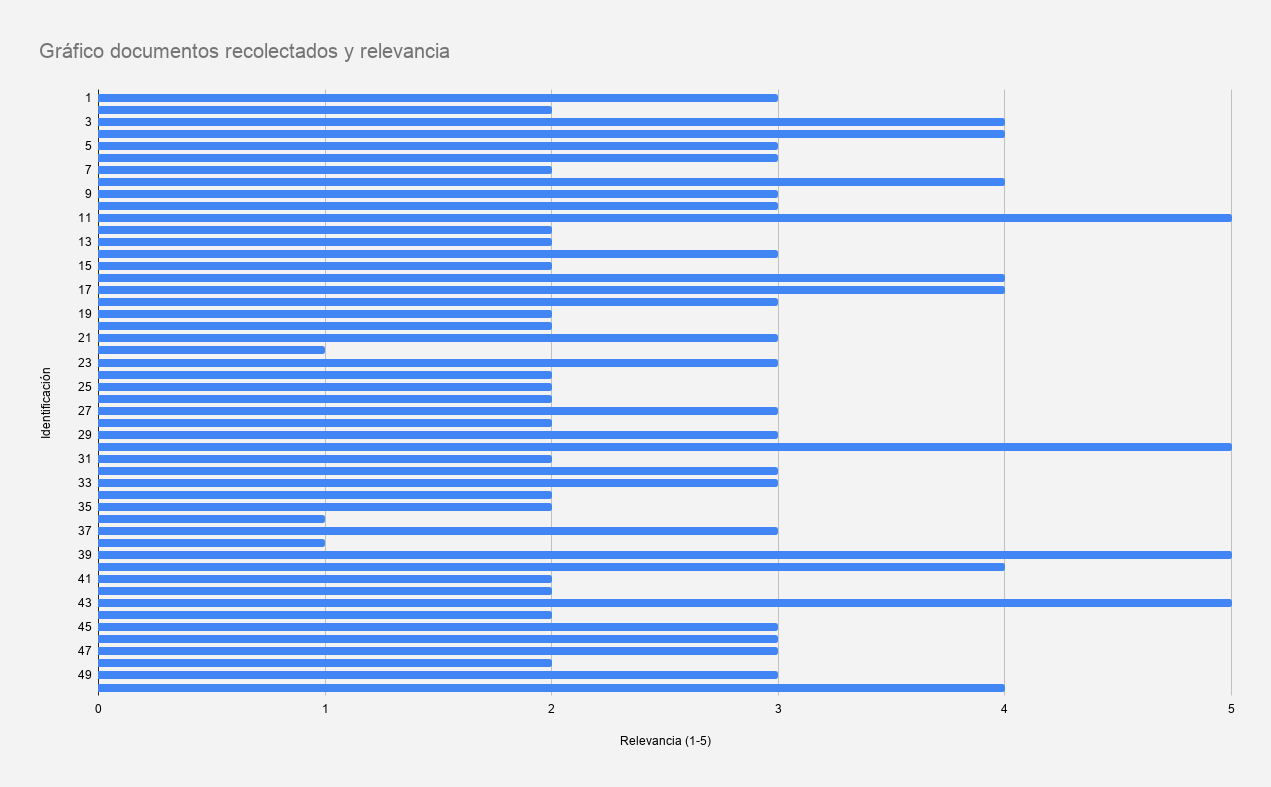
\includegraphics[width=6in,height=3.3in]{Images/GraficoPapers.png}
	    \caption{Relevancia documentos recolectados}
	    Fuente: Elaboración propia
        \label{fig:section}
	\end{Center}
\end{figure}

\begin{justify}
Entre los más relevantes se encuentra BERT (Bidirectional Encoder Representations from Transformers), una técnica de aprendizaje automático basada en Transformer para la formación previa del Procesamiento del Lenguaje Natural (PLN) desarrollada por Google []. Se puede evidenciar que la técnica BERT está presente en los documentos considerados más relevantes y en una cantidad importante de ellos, esto se debe a que los resultados obtenidos en los experimentos realizados por los autores de los artículos son prometedores.
\end{justify}

\begin{justify}
Del mismo modo GPT-2 (Generative Pre-trained Transformer 2), una inteligencia artificial de código abierto creada por OpenAI que  utiliza el aprendizaje profundo para diferentes tareas (Traducción, responder preguntas, resumir pasajes y generar resultados de texto), se encuentra citada en repetidas ocasiones, siendo el más prometedor entre los diferentes tipos de modelos propuestos en los artículos. Su sucesor GPT-3 no ha sido considerado como opción viable debido al acceso restringido a la API y al objetivo al que está enfocado su uso.
\end{justify}


\begin{justify}
En cada documento analizado se logró recopilar las diferentes técnicas de Procesamiento de Lenguaje Natural con el fin de conocer en detalle la construcción de los modelos propuestos o investigaciones presentadas (teoría). Por tanto a continuación se describen las técnicas de PLN utilizadas según la información recopilada en la tabla para las tareas de generación de texto y respuesta a preguntas.
\end{justify}

\begin{itemize}
	\item \textbf{Tokenization:} La tokenización es el proceso de demarcar y posiblemente clasificar secciones de una cadena de caracteres de entrada. Los tokens resultantes luego se pasan a otra forma de procesamiento. El proceso se puede considerar una subtarea de analizar la entrada [].\par

	\item \textbf{NLP Lower-Case}\par

	\item \textbf{StopWords Pre-Processing:} Palabras vacías es el nombre que reciben las palabras sin significado como artículos, pronombres, preposiciones, etc. que son filtradas antes o después del procesamiento de datos en lenguaje natural []. \par

    \item \textbf{Stemming:} Cortar el final o el comienzo de una palabra, teniendo en cuenta una lista de prefijos y sufijos comunes que se pueden encontrar en una palabra flexionada []. \par
    
    \item \textbf{Lemmatization:} Generalmente se refiere a hacer las cosas correctamente con el uso de un vocabulario y análisis morfológico de palabras, normalmente con el objetivo de eliminar solo las terminaciones flexivas y devolver la forma base o de diccionario de una palabra, lo que se conoce como lema []. \par
    
    \item \textbf{StopWords Pre-Processing:} Palabras vacías es el nombre que reciben las palabras sin significado como artículos, pronombres, preposiciones, etc. que son filtradas antes o después del procesamiento de datos en lenguaje natural []. \par
    
    \item \textbf{PoS Tagging (part-of-speech tagging):} Es el proceso de marcar una palabra en un texto (corpus) como correspondiente a una parte particular del discurso, basado tanto en su definición como en su contexto [].  \par
    
    \item \textbf{Term Frequency:} frecuencia de término (o sea, la frecuencia de ocurrencia del término en la colección de documentos), es una medida numérica que expresa cuán relevante es una palabra para un documento en una colección. []. \par
    
    \item \textbf{Word Embedding:} La incrustación de palabras es cualquiera de un conjunto de técnicas de aprendizaje de características y modelado del lenguaje en el procesamiento del lenguaje natural (PNL) donde las palabras o frases del vocabulario se asignan a vectores de números reales []. \par
    
    \item \textbf{Bag of words:} El modelo de bolsa de palabras es una representación simplificada utilizada en el procesamiento del lenguaje natural y la recuperación de información (IR). En este modelo, un texto (como una oración o un documento) se representa como la bolsa (multiset) de sus palabras, sin tener en cuenta la gramática e incluso el orden de las palabras, pero manteniendo la multiplicidad []. \par
    
    \item \textbf{Masked LM (MLM):} El modelado de lenguaje enmascarado es una tarea de rellenar espacios en blanco, en la que un modelo usa las palabras de contexto que rodean un símbolo de máscara para intentar predecir cuál debería ser la palabra enmascarada []. \par
    
    \item \textbf{Next Sentence Prediction (NSP):} En el proceso de entrenamiento de BERT, el modelo recibe pares de oraciones como entrada y aprende a predecir si la segunda oración del par es la oración subsiguiente en el documento original []. \par
    
    \item \textbf{N-gram:} Un n-grama es una secuencia contigua de n elementos de una muestra dada de texto o habla. Los elementos pueden ser fonemas, sílabas, letras, palabras o pares de bases según la aplicación. Los n-gramas normalmente se recopilan de un texto o corpus de voz []. \par
    
    \item \textbf{Named Entity Recognition (NER):} El reconocimiento de entidad con nombre ( NER ) (también conocido como identificación de entidad (con nombre) , fragmentación de entidad y extracción de entidad ) es una subtarea de extracción de información que busca ubicar y clasificar las entidades con nombre mencionadas en texto no estructurado en categorías predefinidas como persona nombres, organizaciones, ubicaciones, códigos médicos , expresiones de tiempo, cantidades, valores monetarios, porcentajes, etc. [].
\end{itemize}\par


\begin{justify}
Para la generación de preguntas en la mayoría de modelos se utiliza SQuAD (Stanford Question Answering Dataset) para entrenar y evaluar los modelos. SQuAD es un conjunto de datos de comprensión de lectura, que consta de preguntas planteadas por los trabajadores de la red en un conjunto de artículos de Wikipedia, donde la respuesta a cada pregunta es un segmento de texto, o un intervalo, del pasaje de lectura correspondiente, o la pregunta podría ser incontestable [].
\end{justify}

\begin{justify}
Gracias a la revisión del estado del arte y recolección de información presentada en la tabla es posible tener una base sólida en la elección de técnicas y modelos a utilizar en el trabajo de grado actual (generación de exámenes de Inglés).
\end{justify}

\begin{justify}
Adicionalmente, una vez obtenida las fuentes teóricas, se recopiló información de manera más específica sobre algoritmos que se basan en la teoría presente en la mayoría de documentos, para este propósito también se realiza una tabla asociada a 10 algoritmos de código abierto disponible en repositorios o plataformas reconocidas como Hugging Face [].
\end{justify}

\begin{justify}
Después de realizar una búsqueda exhaustiva de algoritmos de código libre disponibles en la Web que fueran potencialmente útiles para cumplir el primer objetivo propuesto, se puede concluir que, los modelos basados en Transformers ofrecen resultados de vanguardia tanto para la tarea de generación de texto como para la tarea de respuesta a preguntas. 
\end{justify}

\subsection{Resultados}
\begin{justify}
Tras realizar un análisis profundo sobre los artículos y algoritmos recolectados se describe a continuación los algoritmos seleccionados para la implementación en el prototipo web:

\begin{itemize}
    \item \textbf{Generación de texto}\\
    Para el algoritmo de generación de texto se seleccionó GPT-2 de Hugging Face [] principalmente por la diferencia de rendimiento en comparación con los otros algoritmos recopilados. Dicha diferencia representa casi el doble de tiempo de ejecución en igualdad de condiciones (entradas). Dado que la comparación se redujo a dos algoritmos, el de Hugging Face (GPT-2) y un algoritmo encontrado en GitHub llamado GPT2-Pytorch [], ambos están claramente basados en GPT-2 lo cual implica que los textos generados sean similares al modelo original GPT-2 y que la diferencia se defina por el rendimiento de generación de texto.
    
    El algoritmo proporcionado por Hugging Face es oficial respecto a GPT2-Pytorch que es una modificación de GPT-2 hecha por un desarrollador de la comunidad, de allí las diferencias en algunos aspectos como la calidad de los resultados, esto se debe a que, Hugging Face es un proveedor de código abierto reconocido en el campo de Procesamiento de Lenguaje Natural (PLN).
    
    Se realizaron encuestas a un docente de Inglés con el fin de obtener una evaluación de un experto en cuanto a la calidad de los textos generados por ambos algoritmos, se compararon tiempos de respuesta para comparar el rendimiento, se tuvieron en cuenta las limitaciones y otros detalles, finalmente, los resultados obtenidos favorecieron a GPT-2 Hugging Face.
    
    \item \textbf{Generación de preguntas y respuestas}\\
    Para la selección del algoritmo de generación de preguntas y respuestas, se compararon dos algoritmos de código abierto para esta tarea, sin embargo, desde un inicio uno de los algoritmos presentaba mayor potencial de acuerdo al propósito del proyecto, ya que, de los recolectados es el único algoritmo capaz de generar preguntas y respuestas de opción múltiple y de oraciones (preguntas abiertas), es decir dos tipos de preguntas.
    
    El tipo de preguntas es un factor importante para el propósito del proyecto, ya que, a mayor tipo de preguntas más posibilidades de generar exámenes variados para los estudiantes.
    
    De acuerdo a las pruebas y posterior análisis realizado entre ambos algoritmos inicialmente seleccionados, se decidió seleccionar finalmente el algoritmo encontrado en GitHub llamado Question Generator [], debido a todas las ventajas obtenidas respecto a el propósito del proyecto expuestas anteriormente.
\end{itemize}

    La justificación de selección de algoritmos completa se encuentra en los anexos.
\end{justify}
\end{document}